\documentclass{article}

\usepackage{graphicx}
\usepackage{amsmath}
\usepackage{booktabs}
\usepackage{float}
\usepackage[dvipsnames]{xcolor}
\usepackage{listings}
\usepackage{adjustbox}
\usepackage[
	a4paper,
	left=2.5cm,
	right=2.5cm,
	top=2.5cm,
	bottom=2.5cm,
	headheight=14pt,
	headsep=0.6cm,
	footskip=1cm
]{geometry}
\usepackage{fancyhdr}

\definecolor{nbbg}{HTML}{F7F8FA}
\definecolor{nbframe}{HTML}{D9DEE8}
\definecolor{nbkeyword}{HTML}{1F4E79}
\definecolor{nbstring}{HTML}{A31515}
\definecolor{nbcomment}{HTML}{2E8B57}
\definecolor{nbnumbers}{HTML}{6A737D}

\lstdefinestyle{nbpython}{
	language=Python,
	backgroundcolor=\color{nbbg},
	basicstyle=\ttfamily\small,
	keywordstyle=\color{nbkeyword}\bfseries,
	stringstyle=\color{nbstring},
	commentstyle=\color{nbcomment}\itshape,
	numbers=left,
	numberstyle=\tiny\color{nbnumbers},
	numbersep=8pt,
	frame=single,
	rulecolor=\color{nbframe},
	breaklines=true,
	showstringspaces=false,
	tabsize=4,
	columns=fullflexible
}

\providecommand{\tightlist}{%
	\setlength{\itemsep}{0pt}\setlength{\parskip}{0pt}%
}
\providecommand{\pandocbounded}[1]{%
	\adjustbox{max width=0.8\linewidth,max totalheight=0.65\textheight}{#1}%
}

\pagestyle{fancy}
\fancyhf{}
\fancyhead[L]{ 12-PHY-BIPGP2 General Physics Laboratory 2}
\fancyfoot[R]{ Affan Kaknjo, Andrea Pokrajčić \thepage}
\renewcommand{\headrulewidth}{0.4pt}
\renewcommand{\footrulewidth}{0.4pt}

\setlength{\parindent}{0pt}
\setlength{\parskip}{0.8em}

\fancypagestyle{plain}{
	\fancyhf{}
	\fancyhead[L]{ 12-PHY-BIPGP2 General Physics Laboratory 2}
	\fancyfoot[R]{ Affan Kaknjo, Andrea Pokrajčić \thepage}
	\renewcommand{\headrulewidth}{0.4pt}
	\renewcommand{\footrulewidth}{0.4pt}
}

\begin{document}

\title{Introduction to General Physics Laboratory 2 (Template)}
\author{Affan Kaknjo (50\%), Andrea Pokrajčić (50\%)}
\date{01.01. 2001.}
\maketitle

\section{Tasks}

\subsection{Task 1}

Measure the voltage-current characteristics of a real voltage source by
varying the load resistor \(R_L\). Determine the internal resistance
\(R_i\), the no-load voltage (electromotive force, emf) \(U_q\) and the
short-circuit current \(I_k\) by fitting.

\subsection{Task 2}

From the data of Task 1 calculate the electrical power dissipated by the
load resistor. Determine the internal resistance, the electromotive
force and the maximum power of the voltage source by nonlinear data
fitting in the \(P-R_a\) diagram. Compare these results with those from
Task 1.

\subsection{Task 3}

Measure the voltage-current characteristic of a solar cell by varying
the load resistance RL. Plot the \(P-R_a\) diagram and determine the
operating point and the power generated at this point.

\begin{itemize}
\tightlist
\item
  Subtask 1
\item
  Subtask 2
\item
  Subtask 3
\end{itemize}

\subsection{Task 2}

\section{Theoretical overview}

A real voltage source can be modeled as an ideal electromotive force
(emf) \(U_q\) in series with an internal resistance \(R_i\). The terminal
voltage \(U_k\) across the source depends on the current \(I\) drawn by the
load resistor \(R_L\).


\begin{equation}
U_k = U_q - I \, R_i
\label{nb2tex:eq:1}
\end{equation}

The short-circuit current \(I_k\)(when \(U_k = 0\)) is therefore:


\begin{equation}
I_k = \frac{U_q}{R_i}
\label{nb2tex:eq:2}
\end{equation}

When no current flows (\(I = 0\)), the terminal voltage equals the emf:


\begin{equation}
U_k = U_q
\label{nb2tex:eq:3}
\end{equation}

This linear relationship between \(U_k\) and \(I\) allows one to determine
both \(R_i\) and \(U_q\) by fitting a straight line to the measured
voltage-current data.

\subsection{Plot}

This is an example of plotting.


\begin{lstlisting}[style=nbpython]
import numpy as np
import matplotlib.pyplot as plt

x = np.linspace(0, 10, 100)
y = np.sin(x)

for i in range (3):
    plt.plot(x, y)
    plt.title("Sine Wave")
    plt.show()
\end{lstlisting}


\begin{figure}[H]
\centering
\adjustbox{max width=0.8\linewidth,max totalheight=0.65\textheight}{%
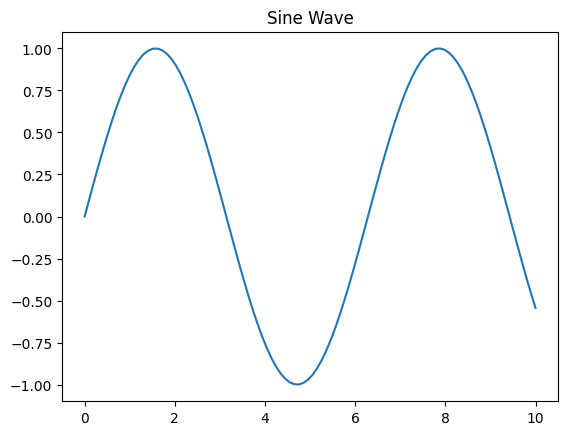
\includegraphics{figures/fig_0.png}%
}
\caption{Generated figure}
\label{nb2tex:fig:1}
\end{figure}


\begin{figure}[H]
\centering
\adjustbox{max width=0.8\linewidth,max totalheight=0.65\textheight}{%
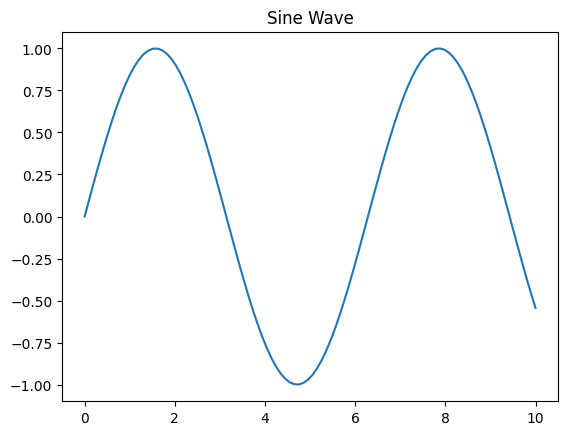
\includegraphics{figures/fig_1.png}%
}
\caption{Generated figure}
\label{nb2tex:fig:2}
\end{figure}


\begin{figure}[H]
\centering
\adjustbox{max width=0.8\linewidth,max totalheight=0.65\textheight}{%
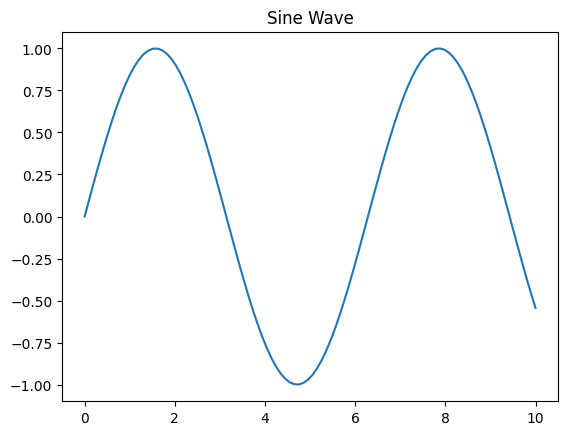
\includegraphics{figures/fig_2.png}%
}
\caption{Generated figure}
\label{nb2tex:fig:3}
\end{figure}

\subsection{Table}


\begin{lstlisting}[style=nbpython]
import pandas as pd

df = pd.DataFrame({
    "A": [1, 2, 3],
    "B": [4, 5, 6]
})
print(df)
\end{lstlisting}


\begin{table}[H]
\centering
\caption{Generated table}
\label{nb2tex:tbl:1}
\vspace{6pt}

\begin{tabular}{ll}
\toprule
A & B \\
\midrule
1 & 4 \\
2 & 5 \\
3 & 6 \\
\bottomrule
\end{tabular}
\end{table}

What about this table?


\begin{table}[H]
\centering
\caption{Generated table}
\label{nb2tex:tbl:2}
\vspace{6pt}

\begin{tabular}{ll}
\toprule
This & is \\
\midrule
a & table \\
\bottomrule
\end{tabular}
\end{table}

\subsubsection{Table with equations in cells}

The following table includes inline equations in cells, including
absolute value notation with a pipe character:


\begin{table}[H]
\centering
\caption{Generated table}
\label{nb2tex:tbl:3}
\vspace{6pt}

\begin{tabular}{lll}
\toprule
Quantity & Expression & Note \\
\midrule
Ohm's law current & $I = \frac{U}{R}$ & Linear relation \\
Load power & $P = I^2 R$ & Resistive load \\
Absolute value example & $|x| = \sqrt{x^2}$ & Contains pipe symbol in math \\
\bottomrule
\end{tabular}
\end{table}

To get around this, we will define three parameters for fitting as
follows: \(a = R_{sp}C\), \(b=RC\) and \(c=LC\). If we rewrite eq. (13)
with the parameter swap we end up with eq. (14).


\end{document}
